\chapter{Results and Inferences}

In this chapter we look at the various results of the simulations our models have gone through. We begin by showing that the system parameter, \acrshort{ber} is within the required limits (less than $10^{-5}$) and also discuss the time taken to transmit $10^6$ bits in the various schemes. We also compare and contrast the results obtained across different schemes and draw conclusions.

\section{Parameters for Simulations}
The common channel parameters for all simulations is as follows
\begin{itemize}
\item In all simulations the noise power spectral density is -80 dBm/Hz
\item The distance between the transmitting and receiving antenna is 1km
\item The gain of the \acrshort{bs} antenna is 8 and \acrshort{ue} antenna is taken as 1
\item A total of $10^6$ bits are transmitted in all cases
\item The maximum number of bits that can be loaded on a subchannel in case of tone loading operation being performed at the transmitter is 20 bits.
\item The number of subchannels is taken to be 256.
\item The power input to the transmitter is 1 mW.
\end{itemize}

Apart from these there are certain randomized parameters such as the \gls{rayleigh fading} coefficient and the noise signal which is additive white Gaussian in nature.


\section{SISO System Results}
The result for the \acrshort{siso} simulation is shown in figure \ref{fig:siso system performance}. The \acrshort{ber} is observed to be $0$, which is within the expected range. Also, the total power deviation due to rounding of the number of bits per tone is $-0.95131$ dB which is less than our threshold value of $\pm 2$ dB.\\
We observe in figure \ref{fig:siso tone loading} that the subchannels with higher \acrshort{snr} have more bits loaded onto them which is the expected behavior of our tone loading algorithm.\\
Since we have only one antenna path to transmit $10^6$ bits, we need a total of $1643$ cycles of transmitting bits as per the tone loading profile in \ref{fig:siso tone loading}. We shall see how using \acrshort{mimo} systems improve this rate.

\begin{figure}[!htbp]
\centering
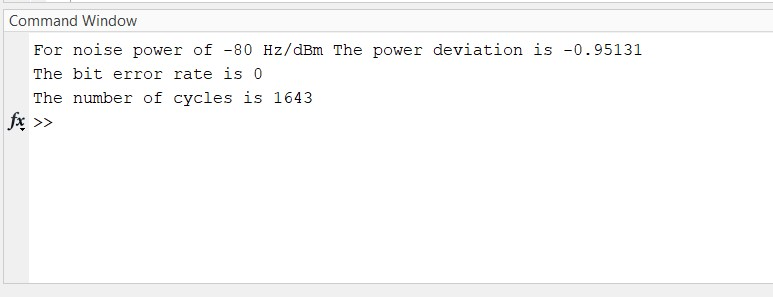
\includegraphics[scale=1]{Chapter 4/Figures/SISO System Performance}
\caption[SISO Tone Loading]{The performance of our SISO system. The number of cycles taken to transmit the bits is of particular importance to us.}
\label{fig:siso system performance}
\end{figure}

\begin{figure}[!htbp]
\centering
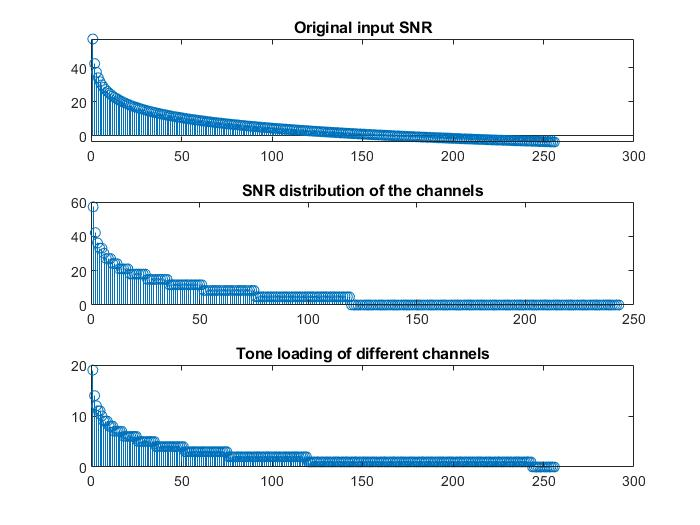
\includegraphics[scale=0.7]{Chapter 4/Figures/SISO Tone Loading}
\caption[SISO Tone Loading]{The tone loading profile of various subchannels for SISO mode.}
\label{fig:siso tone loading}
\end{figure}

\section{SIMO System Results}
The result for the \acrshort{simo} simulation is shown in figure \ref{fig:simo system performance}. The \acrshort{ber} is observed to be $0$, which is within the expected range. Also, the total power deviation due to rounding of the number of bits per tone is $-1.82$ dB which is less than our threshold value of $\pm 2$ dB.\\
We observe in figure \ref{fig:simo tone loading} that the subchannels with higher \acrshort{snr} have more bits loaded onto them which is the expected behavior of our tone loading algorithm.\\
To transmit $10^6$ bits, we need a total of $1051$ cycles of transmitting bits as per the tone loading profile in \ref{fig:simo tone loading}. This is done again in diversity mode. We shall see how using \acrshort{mimo} systems improve this rate.

\begin{figure}[!htbp]
\centering
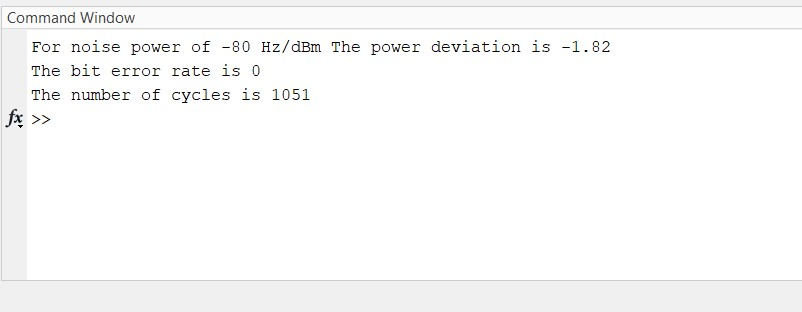
\includegraphics[scale=1]{Chapter 4/Figures/SIMO System Performance}
\caption[SIMO Tone Loading]{The performance of our SIMO system. The number of cycles taken to transmit the bits is of particular importance to us.}
\label{fig:simo system performance}
\end{figure}

\begin{figure}[!htbp]
\centering
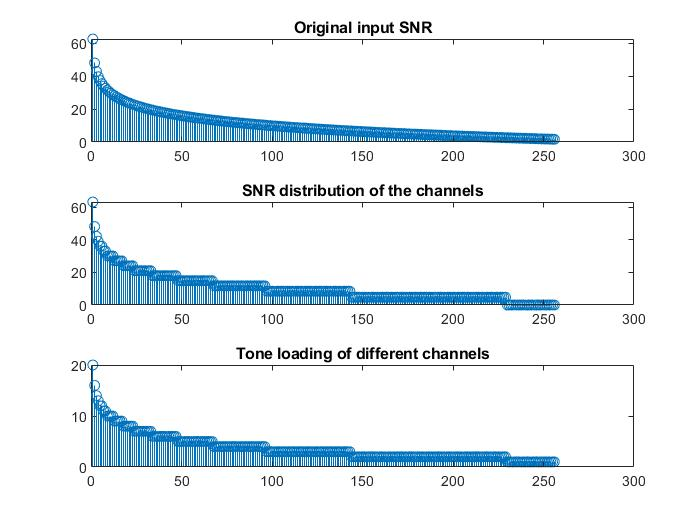
\includegraphics[scale=0.7]{Chapter 4/Figures/SIMO Tone Loading}
\caption[SIMO Tone Loading]{The tone loading profile of various subchannels for SIMO mode.}
\label{fig:simo tone loading}
\end{figure}

\section{MISO System Results}
The result for the \acrshort{miso} simulation is shown in the figure \ref{fig:miso system performance}. The \acrshort{ber} is observed to be $0$, which is within the expected range. We do not perform any tone loading as we use a Alamouti precoding scheme. It takes only $98$ cycles to transmit the $10^6$ bits.

\begin{figure}[!htbp]
\centering
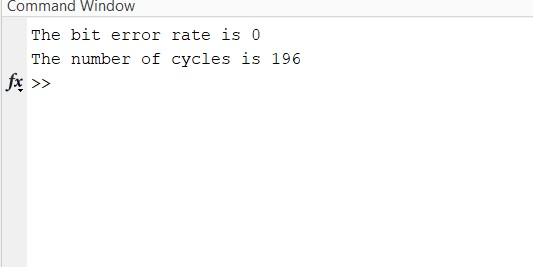
\includegraphics[scale=1]{Chapter 4/Figures/MISO System Performance}
\caption{MISO System Performance.}
\label{fig:miso system performance}
\end{figure}

\section{MIMO System Results}

\subsection{MIMO Diversity Case}
The result for the \acrshort{mimo} simulation in diversity case is shown in figure \ref{fig:mimo system performance diversity}. The \acrshort{ber} is observed to be $0$, which is within the expected range. Also, the total power deviation due to rounding of the number of bits per tone is $-1.3892$ dB which is less than our threshold value of $\pm 2$ dB.\\
We observe in figure \ref{fig:mimo tone loading diversity} that the subchannels with higher \acrshort{snr} have more bits loaded onto them which is the expected behavior of our tone loading algorithm.\\
Although we have many antenna paths to transmit $10^6$ bits, since we are operating in diversity mode we need a total of $1303$ cycles of transmitting bits as per the tone loading profile in \ref{fig:mimo tone loading diversity}. We shall see how operating \acrshort{mimo} in multiplexing mode can vastly improve this system performance.

\begin{figure}[!htbp]
\centering
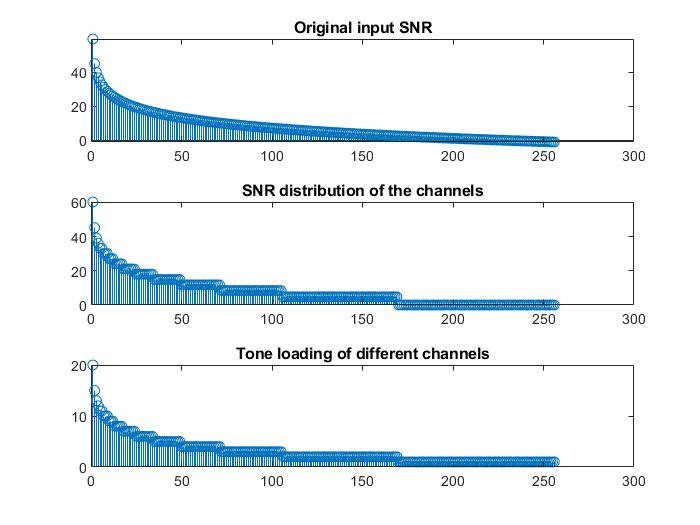
\includegraphics[scale=0.7]{Chapter 4/Figures/MIMO Tone Loading Diversity}
\caption[MIMO Tone Loading in Diversity Case]{The tone loading profile of various subchannels for MIMO in diversity mode.}
\label{fig:mimo tone loading diversity}
\end{figure}

\begin{figure}[!htbp]
\centering
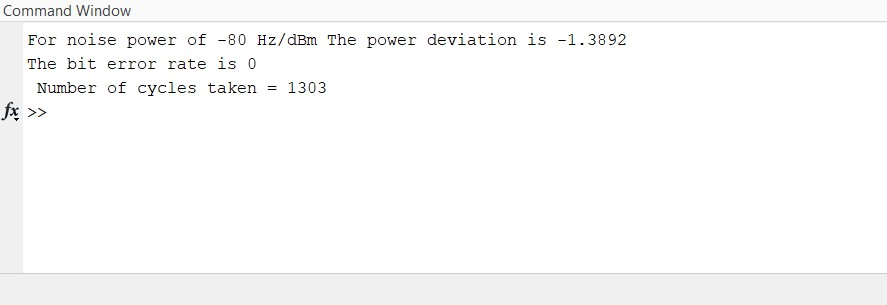
\includegraphics[scale=1]{Chapter 4/Figures/MIMO System Performance Diversity}
\caption[MIMO System Performance in Diversity Case]{The performance of our MIMO system. The number of cycles taken to transmit the bits is of particular importance to us.}
\label{fig:mimo system performance diversity}
\end{figure}

\subsection{MIMO Multiplexing Case}

The result for the \acrshort{mimo} simulation in multiplexing case is shown in figure \ref{fig:mimo system performance multiplexing}. The \acrshort{ber} is observed to be $0$, which is within the expected range. Also, the total power deviation due to rounding of the number of bits per tone is $-0.65038$ dB which is less than our threshold value of $\pm 2$ dB.\\
We observe in figure \ref{fig:mimo tone loading multiplexing} that the subchannels with higher \acrshort{snr} have more bits loaded onto them which is the expected behavior of our tone loading algorithm.\\
Since we have many antenna paths to transmit $10^6$ bits, we only $797$ cycles of transmitting bits as per the tone loading profile in \ref{fig:mimo tone loading diversity}. As we see, in the multiplexing case, the number of cycles have reduced considerably directly interfering higher data rates.

\begin{figure}[!htbp]
\centering
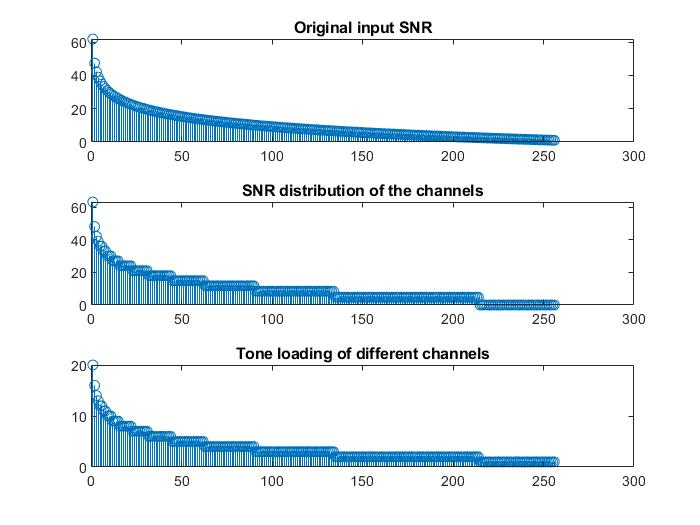
\includegraphics[scale=0.7]{Chapter 4/Figures/MIMO Tone Loading Multiplexing}
\caption[MIMO Tone Loading in Multiplexing Case]{The tone loading profile of various subchannels for MIMO in diversity mode.}
\label{fig:mimo tone loading multiplexing}
\end{figure}

\begin{figure}[!htbp]
\centering
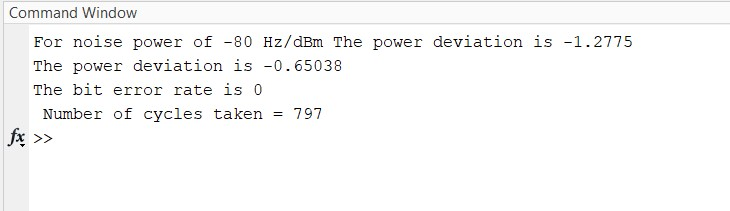
\includegraphics[scale=1]{Chapter 4/Figures/MIMO System Performance Multiplexing}
\caption[MIMO System Performance in Multiplexing Case]{The performance of our MIMO system. The number of cycles taken to transmit the bits is of particular importance to us.}
\label{fig:mimo system performance multiplexing}
\end{figure}

\subsection{MIMO Multiplexing with Inverse Channel Estimation Precoder}

The result for the \acrshort{mimo} simulation for multiplexing case with inverse channel estimation precoder is shown in the figure \ref{fig:mimo system performance inverse channel estimation}. The \acrshort{ber} is observed to be $0$, which is within the expected range. We do not perform any tone loading as we use a Inverse Channel Estimation precoding scheme. It takes only $98$ cycles to transmit the $10^6$ bits. We notice how by using suitable precoding the number of cycles reduce drastically.

\begin{figure}[!htbp]
\centering
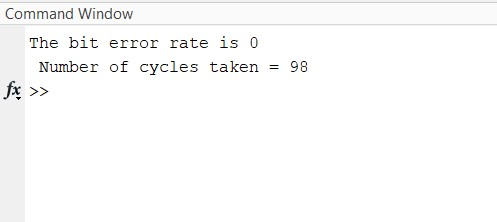
\includegraphics[scale=1]{Chapter 4/Figures/MIMO System Performance Inverse Channel Estimation}
\caption{MIMO System Performance with Inverse Channel Estimation Precoder.}
\label{fig:mimo system performance inverse channel estimation}
\end{figure}

\subsection{MIMO Multiplexing with Singular Value Decomposition Precoder}

The result for the \acrshort{mimo} simulation for multiplexing case with singular value decomposition precoder is shown in the figure \ref{fig:mimo system performance singular value decomposition}. The \acrshort{ber} is observed to be $0$, which is within the expected range. We do not perform any tone loading as we use a Singular Value Decomposition precoding scheme. It takes only $98$ cycles to transmit the $10^6$ bits. We notice how by using suitable precoding the number of cycles reduce drastically.

\begin{figure}[!htbp]
\centering
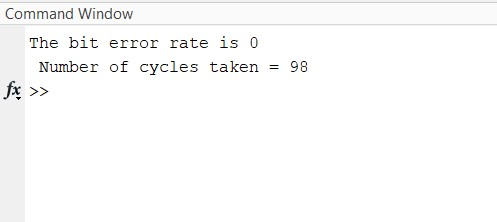
\includegraphics[scale=1]{Chapter 4/Figures/MIMO System Performance Inverse Channel Estimation}
\caption{MIMO System Performance with Singular Value Decomposition Precoder.}
\label{fig:mimo system performance singular value decomposition}
\end{figure}

\section*{Summary}
In this section we discussed the results of the simulations of our system in various configurations. We clearly see that data rates increase with multiplexing mode and also with precoding. Finally, in the last section we conclude our report and talk about the future scope of the report and how further improvements can be made to our system.




